\section{Stovepipe System}

\subsection{Form \& Causes}
Stovepipe System Anti-Pattern occur within one system. Two definitions can be found:
\begin{itemize}
\item Term describes system developed to solve a specific problem and containing data that cannot be easily shared with other systems \cite{c2com}.
\item System where no abstraction layers are used to communicate between subsystem which results in situation where everything is connected with everything \cite{Virtual,Solutions}.
\end{itemize}
The first one is more general and applies to all stovepipe anti-patterns.
The second one will be further discussed in next chapters.

It happens in systems which integrates different subsystems to achieve they goal. But direct causes of this anit-pattern is no architectural vision which leads to lack of already mentioned abstraction in the system providing tight coupling between implemented subsystems \cite{SurvivalGuide}.


\subsection{Distinction}

When describing stovepipe anti-patterns the clear distinction between them should be provided. Example difference are listed in \hyperref[tab:Distinction]{figure \ref{tab:Distinction}}.

\def\arraystretch{1.6}
\begin{center}
\begin{figure}[!h]
	\begin{tabular}{|p{.48\linewidth}|p{.48\linewidth}|}
	    \hline
	    Stovepipe Enterprise & Stovepipe System \\
	    \hline
	    Multiple systems & One system \\
	    Lack of common layer between systems & Lack of common abstract layer between subsystems \\
	    Caused by: & Caused by: \\
	    \ - Lack of communication & \ - Lack of architectural vision \\
	    \ - Lack of standards & \  - Tight coupling between classes \\
	    \hline
	\end{tabular}
\caption{Distinction between Stovepipe Enterprise and Stovepipe System}
\label{tab:Distinction}
\end{figure}
\end{center}

\subsection{Symptoms \& Consequences}

One of the main symptoms is difficulty in both modifying the system and describing its architecture. This leads to large semantic gap between architecture documentation and implementation and software will probably not meet the user expectations even when code is comply with the paper requirements \cite{Virtual}. System maintenance will become increasingly costly with both time and money \cite{SurvivalGuide,Virtual,Solutions}. Developers will have to invent workarounds and most attempts to automate system will fail \cite{SurvivalGuide}.

\newpage
\subsection{Example}

Example stovepipe system shown on \hyperref[fig:StovepipeSystemExample]{figure \ref{fig:StovepipeSystemExample}} can be divided into four types of components:
\begin{itemize}
	\item Clients
	\item Scanners
	\item Printers
	\item Databases
\end{itemize}
In the example all subsystems are connected together and there is no abstraction layers between components. Each client has its own code to manage all devices and other clients.

\begin{figure}[!h]
    \centering
    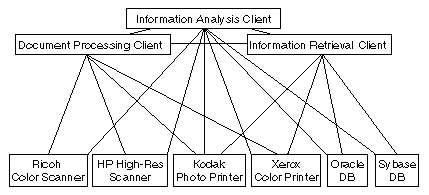
\includegraphics[scale=1.3]{Images/ssexample.png}
    \caption[Stovepipe System Example]{Stovepipe System - example diagram \cite{Solutions}}
    \label{fig:StovepipeSystemExample}
\end{figure}

\subsection{Solution}

\begin{figure}[!h]
    \centering
    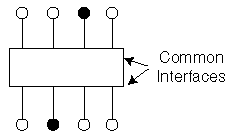
\includegraphics[scale=1]{Images/CommonInterface.png}
    \caption[Interface between subsystems]{Interface between subsystems \cite{Solutions}}
    \label{fig:CommonInterface}
\end{figure}
Refactoring of stovepipe system begins from extracting abstract models for subsystems. Abstract models will allow reuse of code and adding new subsystem will not require code changes in any of clients. Discovering the appropriate abstraction is the key to defining component interfaces. This will model subsystems interoperability without exposing unnecessary differences between subsystems \cite{Solutions}.

Summarizing: non of the subsystems should communicate without abstraction layer.

\newpage

For our example proper abstraction architecture may look like it is shown on \hyperref[fig:StovepipeSystemExampleSolution]{figure \ref{fig:StovepipeSystemExampleSolution}}.
From base graph shown on \hyperref[fig:StovepipeSystemExample]{figure \ref{fig:StovepipeSystemExample}} three types of subsystems interfaces can be extracted along with client interface - because each of the client is also connected with other clients. Those types are:
\begin{itemize}
\item Input devices
\item Output devices
\item Information sources
\end{itemize}
and client interface.

\begin{figure}[!h]
    \centering
    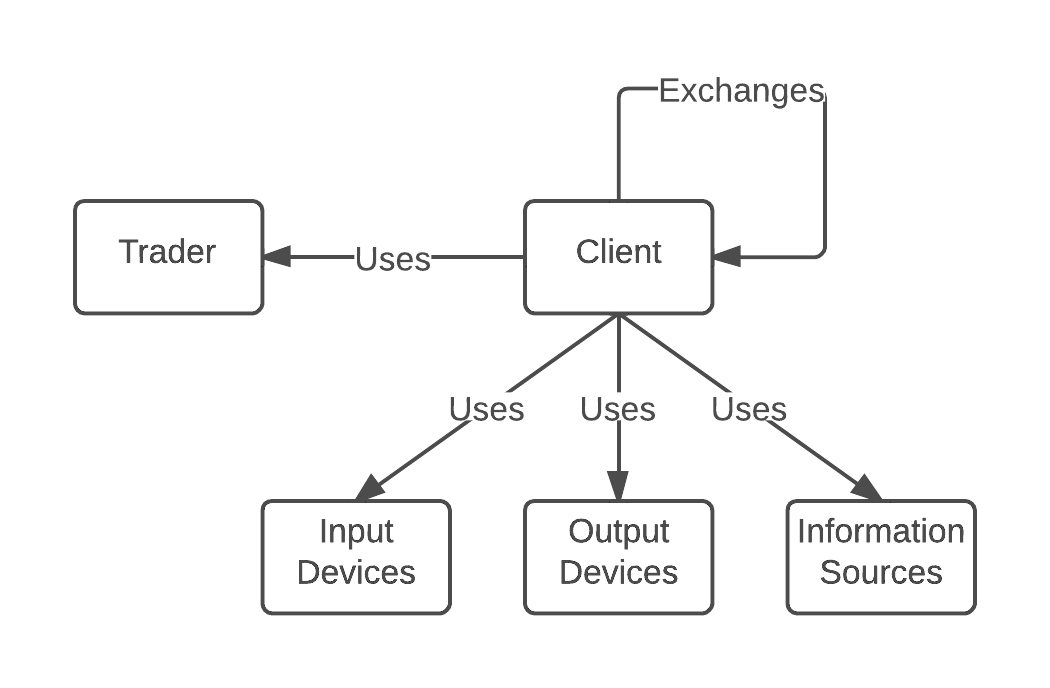
\includegraphics[scale=0.3]{Images/ssexamplesolution.png}
    \caption[Stovepipe System Example Solution]{Stovepipe System - abstraction to example diagram \cite{Solutions}}
    \label{fig:StovepipeSystemExampleSolution}
\end{figure}

There is now direct communication and no tight coupling between components which allows to easily add or remove subsystems and clients.

\subsection{Exceptions}

There are situations which justify this anit-pattern in project. One of those is exploration of new or unknown domain - creating prototypes. Also quick development may end up as stovepipe system but this is acceptable for achieving rapid solutions \cite{SurvivalGuide,Virtual}.